% ----------------------------------------------------------------------------
% BODY/1_esempio.tex -- capitolo di esempio
% Mostra gli elementi piu' comuni: sezioni, citazioni, formule, figure,
% tabelle e riferimenti incrociati. Sostituiscilo con il tuo primo capitolo.
% Convenzione consigliata: un file per capitolo (BODY/2_nome.tex, ...), poi
% aggiungi \include{BODY/2_nome} in main.tex.
% ----------------------------------------------------------------------------
\chapter{Capitolo di esempio}
\label{cap:esempio}

\section{Citazioni e bibliografia}
\label{sec:citazioni}

Le citazioni numeriche si inseriscono con \verb|\cite{chiave}|, dove la chiave
\`e quella definita in \texttt{bibliografia.bib}. Un singolo riferimento appare
come~\cite{wilkinson_fair_2016}; pi\`u riferimenti vengono compattati
automaticamente~\cite{lamport_latex_1994,knuth_texbook_1984}. Anche le risorse
web possono essere citate~\cite{ctan_biblatex}.

\section{Formule}
\label{sec:formule}

Una formula in linea si scrive tra dollari, ad esempio $\bar{x} = \frac{1}{n}\sum_{i=1}^{n} x_i$.
Una formula numerata e richiamabile con \verb|\cref| usa l'ambiente \texttt{equation}:
\begin{equation}
  \mathrm{OR} = \frac{a \cdot d}{b \cdot c}
  \label{eq:odds_ratio}
\end{equation}
come mostra l'\cref{eq:odds_ratio}.

\section{Figure}
\label{sec:figure}

La \cref{fig:esempio} mostra una figura con didascalia e riferimento incrociato:
\`e un esempio di \emph{correlazione spuria}, due serie che si muovono insieme
($r = 0.67$) senza alcun legame causale~\cite{vigen_spurious_2024}. In PDF/A-1b usa
immagini \textbf{senza canale alpha}: vedi il \texttt{README.md}.

\begin{figure}[htbp]
  \centering
  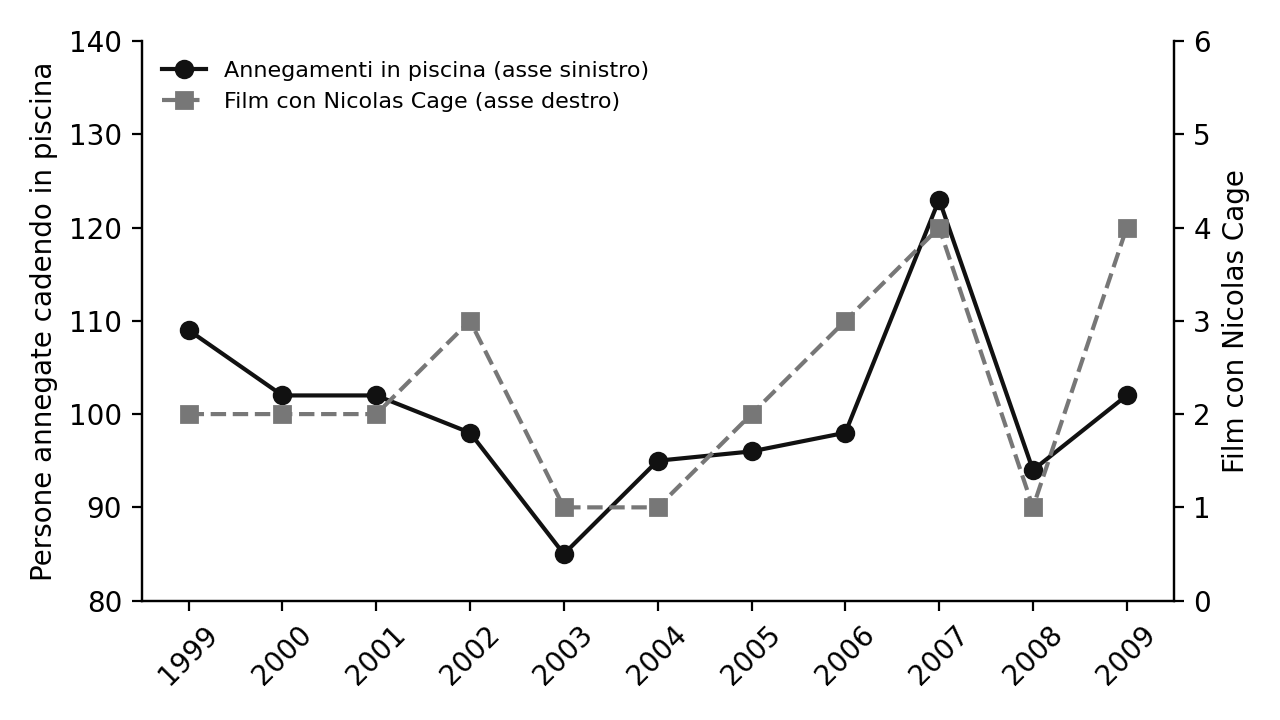
\includegraphics[width=0.8\textwidth]{FIGURE/correlazione_spuria.png}
  \caption{Persone annegate cadendo in piscina e film con Nicolas Cage, 1999--2009
  (correlazione spuria) \cite{vigen_spurious_2024}}
  \label{fig:esempio}
\end{figure}

\section{Tabelle}
\label{sec:tabelle}

La \cref{tab:esempio} usa il pacchetto \texttt{booktabs}, che produce tabelle
pulite con linee orizzontali ben spaziate e senza linee verticali.

\begin{table}[htbp]
  \centering
  \caption{Esempio di tabella (dati fittizi).}
  \label{tab:esempio}
  \begin{tabular}{lrr}
    \toprule
    Gruppo & Soggetti (n) & Eventi (\%) \\
    \midrule
    Gruppo A & 120 & 12.5 \\
    Gruppo B & 118 & 8.5 \\
    \bottomrule
  \end{tabular}
\end{table}

Per i riferimenti interni usa \verb|\label| e \verb|\cref|: vedi l'\cref{app:esempio}
e la \cref{sec:citazioni}.
